%%% File: ./inputs/parts/SENSORIMOTOR_HIERARCHY.tex

%%% %%%%%%%%%%%%%%%%%%%%%%%%% BEGIN SENSORIMOTOR HIERARCHY %%%%%%%%%%%%%%%%%%%%%

Much of the cortex is in the business of learning representations of concepts relevant to survival\footnote{%
%
  The word {\it{perspicacity}} refers to a clarity of perception that enables one to recognize subtle differences between similar physical objects or abstract concepts. It is employed in this context to call attention to the fact that attention, exploration, perception, and prediction are inextricably linked in complex biological systems~\cite{RaoandBallardNATURE-NEUROSCIENCE-99,BarlowNC-89,BaddeleyQJoEP-86,ClarkBBS-13}.}.
%
Perception is the means by which we apprehend and act on the physical realization of the concepts we have learned. It seems obvious that perception serves action. It may not seem so obvious that action serves perception, but the fact is we are almost always moving our head, hands and torso in order to resolve ambiguities in what we see, feeling the shape of unfamiliar objects in order to grasp them firmly and twisting about to see who is behind us calling our name or to get a better idea of where we've come from in order to ensure we can retrace our steps. These are complex sensorimotor activities we depend on every day.

In thinking about physically realizable concepts we think first about what they look, feel, sound and smell like. The sensory cortex is responsible for constructing a hierarchy of representations to characterize such concepts, not to capture everything we sense, but rather to account for what we need to know about concepts to survive. Reconstructing scenes with photographic realism is not what our sensory systems were designed for. Circuits of the primary sensory cortex feed into the circuits of the (unimodal) association sensory cortex that feed into (multimodal) sensory cortex. All of these representations are abstract and yet patterns of regionalization are remarkably preserved within species~\cite{ChenetalNEURON-18,PortuguesetalNEURON-14,KolsteretalJoN-09}.

Concepts arise in patterns of neural activity that account for what we need to know about them, including how they appear to us so we can recognize them, what affordances they offer for us to make use of them and how we might predict their occurrence in decision making. Many of the concepts that are represented in our brains serve to model the dynamics of physical systems that we interact with every day, such as riding a bike, working with tools, opening doors, negotiating stairs and riding escalators in department stores. Just as important, if not more so, are the social dynamics we deal with at work and school with their constantly shifting personal relationships and status rankings. 

If you are a software engineer designing robot control systems, you might give action much the same scrutiny as perception and build a parallel hierarchy of representations that describes the concepts that relate to movement including navigation, articulation and manipulation ranging from servo-motor commands to strategies for moving furniture, but designing or learning these hierarchies independently is generally a bad idea. In mammals, these two hierarchies are tightly coupled to account for how they depend on one another~\cite{FusterPREFRONTAL-CORTEX-15}.

Indeed, determining what sensory representations to learn depends upon and influences what motor representations to learn and {\it{vice versa}}, where we follow the convention of using the term {\it{motor}} as a catchall term for concepts relating to muscles and movement. As pointed out in the introduction, there is evidence to suggest that circuits occurring early in the ventral visual stream code for object-selective features and exhibit large-scale organization characterized by the high-level properties of animacy and object size~\cite{KonkleandCaramazzaJoN-13,LongetalPNAS-18}.

%%% %%%%%%%%%%%%%%%%%%%%%%%%%%%%%%%%%%%%%%%%%%%%%%%%%%%%%%%%%%%%%%%%%%%%%%%%%%%%

%%% Figure~{\urlh{#fig_Coupled_Sensory_Motor_Hierarchy}{\ref{fig_coupled}}}
\begin{figure}
%
  \begin{center} 
%     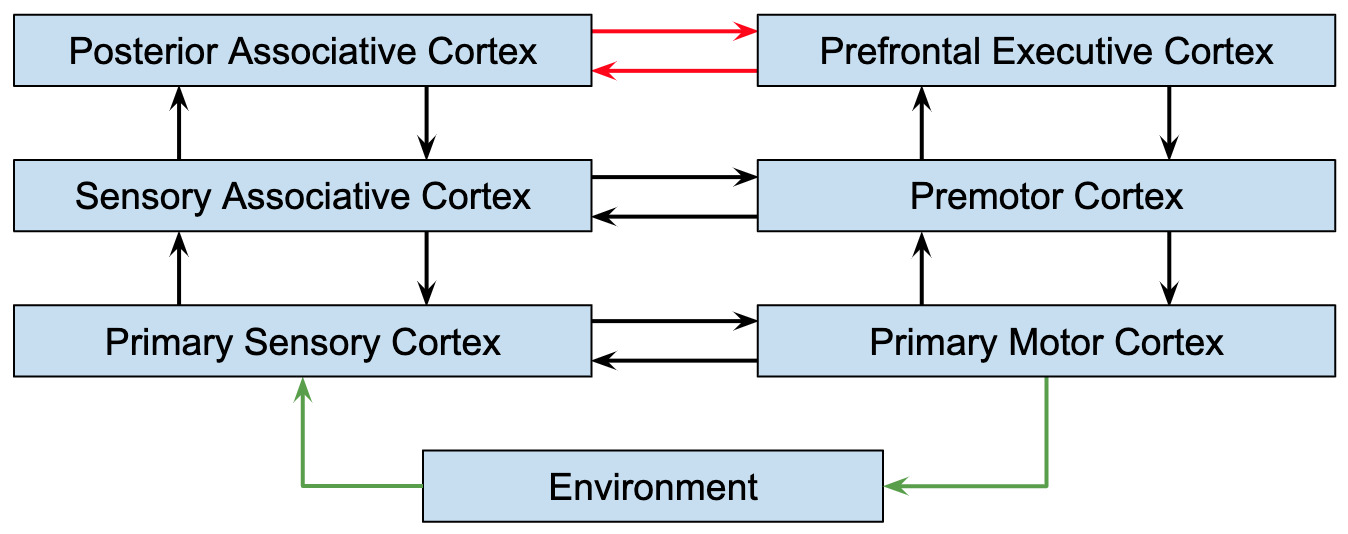
\includegraphics[width=600pt]{./figures/Coupled_Sensory_Motor_Hierarchy.png} %%% 1555 × 635 pixels
    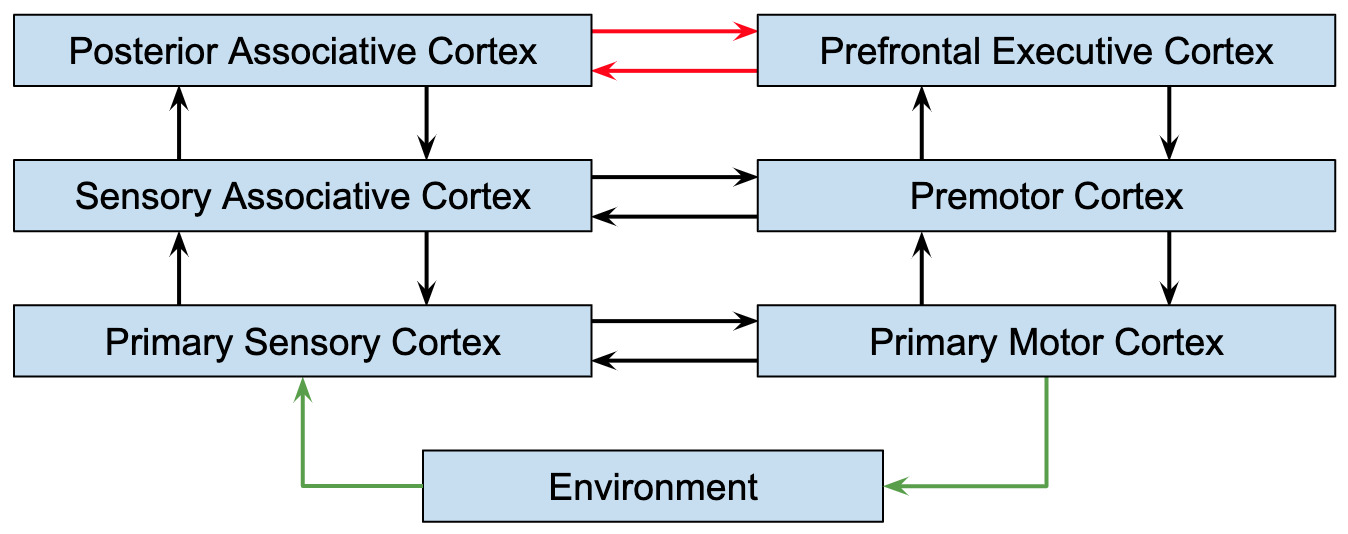
\includegraphics[width=200pt]{./figures/Coupled_Sensory_Motor_Hierarchy.png} %%% 1555 × 635 pixels
  \end{center}
%
  \caption{A simplified block diagram of the cortex. The column on the left represents the posterior cortex including the occipital, temporal and parietal lobes. The column on the right represents the frontal lobe of the cortex corresponding to the primary motor cortex, premotor cortex (association motor cortex) and prefrontal cortex. Green arrows represent interaction with the environment, black arrows represent sensorimotor abstractions and red arrows indicate cognitive activity relating speech, planning and abstract thinking. See the main text for more detail. Adapted from Figure~8.9 in~\cite{FusterPREFRONTAL-CORTEX-15-CHAPTER_8}}
%    
  \label{fig_coupled}
%
\end{figure}

%%% %%%%%%%%%%%%%%%%%%%%%%%%%%%%%%%%%%%%%%%%%%%%%%%%%%%%%%%%%%%%%%%%%%%%%%%%%%%%

Figure~{\urlh{#fig_Coupled_Sensory_Motor_Hierarchy}{\ref{fig_coupled}}} is a simplified block diagram of the cortex organized as two columns. The left column represents the posterior cortex consisting of the occipital, temporal and parietal lobes that are primarily concerned with processing sensory information. The relevant brain areas are summarized in three blocks roughly corresponding to primary sensory cortex, unimodal association cortex and multimodal association cortex stacked so the least abstract concepts are on the bottom and most abstract on the top. The combined area is often referred to as {\it{semantic memory}} and characterized as long-term declarative memory~\cite{BinderandDesaiTiCS-11}. 

The right column represents the frontal lobe of the cortex corresponding to the primary motor cortex, premotor cortex (associative motor cortex) and prefrontal cortex. The primary motor cortex is responsible for creating abstract representations of motor activity throughout the body. The premotor cortex is responsible for integrating sensory and motor abstractions to construct sensorimotor representations. The prefrontal cortex orchestrates cognitive behavior including speech, planning and abstract thinking, and is reciprocally connected to the association areas just mentioned as well subcortical structures including the basal ganglia and hippocampus.

The two columns are connected with one another at multiple levels: by physical interaction with the environment (green arrows), by sensorimotor abstraction and alignment (black arrows), and by cognitive effort in directing activity mediated through subcortical structures (red arrows). This arrangement supports the formation of rich representations that serve a wide range of cognitive function. The sensorimotor connections and feedback through the environment provide an inductive bias to guide learning, ground inference and reduce sample complexity by reducing reliance on labeled data and enabling opportunities for unsupervised learning~\cite{BarlowNC-89}.

Simple as this model of cortical function may seem, it may be one of the most important architectural contributions of neuroscience to the development of artificial intelligence patterned after the human brain. Some of the lessons have already been integrated into the discipline of control theory through exposure to early work in biological cybernetics~\cite{FukushimaBC-80,Lettvinetal59,Jackson1958selected,GibsonPERCEPTION-50,McCullochandPitts43,vonUexk1926theoretical}, but some of the most important lessons impact the application of machine learning in building autonomous embodied systems including robots and digital assistants as alluded to above. 

%%% %%%%%%%%%%%%%%%%%%%%%%%%%% END SENSORIMOTOR HIERARCHY %%%%%%%%%%%%%%%%%%%%%%
